\section{Results}
\label{sec:results}

% Final global set (Jul 2026): A/P curve N=62 (JRC-referenced, best-of adapt/vv,
% de-spiked JRC, reference-noise screened -- 14 unreliable-reference reservoirs
% and 4 flat-pool reservoirs excluded, 1 lacking the fixed-dual export excluded);
% four-way N=47 (additionally requires the retired fixed-dual and fast exports,
% never run for the global-coverage/dip-bin/temperate additions -- this N is not
% meant to match the A/P-curve N, see Methods 3.7.1). Antero re-included 9 Jul 2026
% (was on a stale hardcoded EXCLUDE list predating the reference-noise screen;
% it passes that screen and is part of the trusted N=62 set, so excluding it only
% from the four-way comparison was an inconsistency, not a data-quality reason).
% Figures pulled live from
% analysis/method_comparison_output/ via \graphicspath.

\subsection{A/P predicts SAR monitorability a priori}
\label{sec:res_ap}

Across the 62 globally distributed, reference-quality-screened reservoirs
(Section~\ref{sec:val_global}), the static area-to-perimeter ratio is a strong
predictor of surface-area skill: Spearman $\rho(\text{A/P},\text{KGE}) = 0.51$
($p = 2.7\times10^{-5}$, Figure~\ref{fig:ap_curve}). Skill here is the KGE of the
better of the two per-scene detectors (Section~\ref{sec:res_fourway}). The
relationship behaves as a \emph{ceiling} rather than a simple trend. High-A/P
reservoirs ($\geq$200~m) are reliably tracked (median KGE 0.93, $n=18$),
whereas low-A/P reservoirs ($<$100~m) show both a lower median (0.48, $n=16$)
and a much wider spread, down to negative KGE. Overall 82\% of the reservoirs
reach KGE~$\geq$~0.5.

This is the signature expected if A/P sets the geometric ceiling on
monitorability: compact shorelines leave little room for mixed-pixel error, so
skill is high and stable, whereas elongated, dendritic shorelines merely
\emph{permit} large errors that a second, radiometric axis
(Section~\ref{sec:res_climate}) then determines. The relationship holds for
each detector separately, not only for the best-of series used above:
Spearman $\rho(\text{A/P},\text{KGE}) = 0.41$ for the per-scene SVM alone and
$0.51$ for VV Otsu alone.

\begin{figure}[H]
  \centering
  
\includegraphics[width=0.9\linewidth]{ap_kge_curve_pooled}
  \caption{Surface-area skill (KGE against JRC, best of the two per-scene
  detectors) versus static A/P for the 62 global reservoirs, coloured by which
  detector won. A/P sets a monitorability ceiling: high-A/P reservoirs are
  reliably tracked. Low-A/P reservoirs are permitted, but not guaranteed, large
  errors. Points are labelled by the continent-coded ID listed against each
  reservoir's name in Table~\ref{tab:pilot}.}
  \label{fig:ap_curve}
\end{figure}

Figure~\ref{fig:timeseries_panel} makes this ceiling concrete with sample
monthly series, four reservoirs per A/P band, all with KGE~$>$~0.5. At
high A/P, both detectors track JRC closely, with only minor offsets at the
seasonal extremes. At low A/P, the same KGE~$>$~0.5 threshold is compatible
with a persistent systematic bias, most visibly Songhuaba, where the VV
Otsu series runs some 300--350~ha above JRC throughout while still
correlating well enough to clear the threshold: a reminder that KGE~$>$~0.5
certifies that a detector tracks the reservoir's dynamics, not that its
absolute area is unbiased, and that the bias itself grows as A/P falls,
exactly as the mixed-pixel argument predicts.

\begin{figure}[H]
  \centering
  
\includegraphics[width=\textwidth]{timeseries_panel}
  \caption{Sample monthly water-area series (JRC optical reference vs the
  two per-scene detectors), four reservoirs per static-A/P band, all with
  KGE~$>$~0.5. High-A/P series track JRC tightly; low-A/P series can clear
  KGE~$>$~0.5 while still carrying a large systematic offset (Songhuaba).}
  \label{fig:timeseries_panel}
\end{figure}

\subsection{Per-scene adaptivity matters more than polarisation count}
\label{sec:res_fourway}

The central comparison is the per-scene VV Otsu threshold against the
per-scene dual SVM, evaluated across the full screened set: 62 reservoirs,
59 after excluding three whose SVM export does not share enough common
months with JRC to compute a paired KGE (their VV Otsu series overlaps JRC
without issue, Section~\ref{sec:val_global}). The two are statistically
indistinguishable, overturning the intuitive ``dual-pol beats single-pol''
expectation: a paired Wilcoxon signed-rank test on the 59 finds no
significant difference between them ($p = 0.37$,
Figure~\ref{fig:fourway}d). VV Otsu is nonetheless the better or equal
detector in the majority of reservoirs (it wins 38 of 62,
Figure~\ref{fig:ap_curve}). That majority does not register as a
significant Wilcoxon result, however: the SVM's fewer wins tend to be
larger (median winning margin 0.12 KGE, against 0.08 for Otsu), so a
handful of big SVM wins offsets many small VV wins in the paired,
rank-based test. This same asymmetry is
why the trend line in Figure~\ref{fig:fourway}d tilts above the 1:1 line at
low VV-Otsu skill: the SVM's advantage concentrates in the harder,
low-KGE cases it occasionally rescues, not in a general edge across most
reservoirs. Neither climate zone nor the detector's own baseline accuracy
predicts which reservoirs see the SVM's largest gains
(Section~\ref{sec:disc_limitations}). A dual-polarisation advantage is not
concentrated by A/P either: the difference between the per-scene SVM and
the per-scene Otsu does not depend on it
(Spearman$(\text{A/P},\,\text{KGE}_{\text{SVM}}-\text{KGE}_{\text{Otsu}}) =
-0.14$, $p = 0.36$).

Two further variants, the fixed-2023-training SVM and a
no-vectorisation ``fast'' VV path, only have exports for 47 of the 62 (the
most recent 15-reservoir expansion was run with just the two per-scene
detectors, Section~3.2), so the four-way comparison
(Figure~\ref{fig:fourway}a--c) is restricted to that subset, evaluated on
strictly common months across all four exports (a stricter window than the
pairwise comparison above, so individual KGE values shift slightly).
Ranked by median KGE on it, the order is \emph{per-scene SVM} (0.78) $>$
\emph{per-scene VV Otsu} (0.74) $>$ \emph{VV Otsu without vectorisation}
(0.69) $>$ \emph{fixed-training dual SVM} (0.66). This is the same
margin-driven asymmetry as above, not a reversal of it: within this
subset VV Otsu still wins more often (27 of 47 versus 20 for the SVM), but
the SVM's fewer wins are large enough to lift its median above VV Otsu's.
The fixed-training
dual-polarisation learner ranks \emph{last}, below the single-polarisation
threshold (Figure~\ref{fig:fourway}c), because VV Otsu adapts to every
scene by construction while the fixed SVM does not: per-scene adaptivity
matters more than the number of polarisations. Retraining the SVM per
scene (adapt versus the fixed baseline) wins in 24 of 47 reservoirs, ties
in 7, and loses in 16, but the median improvement is small ($\Delta$KGE
$+0.02$) against a much larger mean improvement ($+0.20$), the same
right-skewed pattern as above: a handful of reservoirs where the fixed
2023 baseline fails badly account for most of the gain, while the typical
reservoir sees only a modest benefit from retraining. Removing the
vectorisation post-processing (the ``fast'' path), separately, does cost
accuracy (median $\Delta$KGE $-0.07$ versus VV Otsu, worse in 32 of 47
reservoirs), so that step is retained. The implications of this parsimony
result are discussed in Section~\ref{sec:discussion}.

\begin{figure}[H]
  \centering
  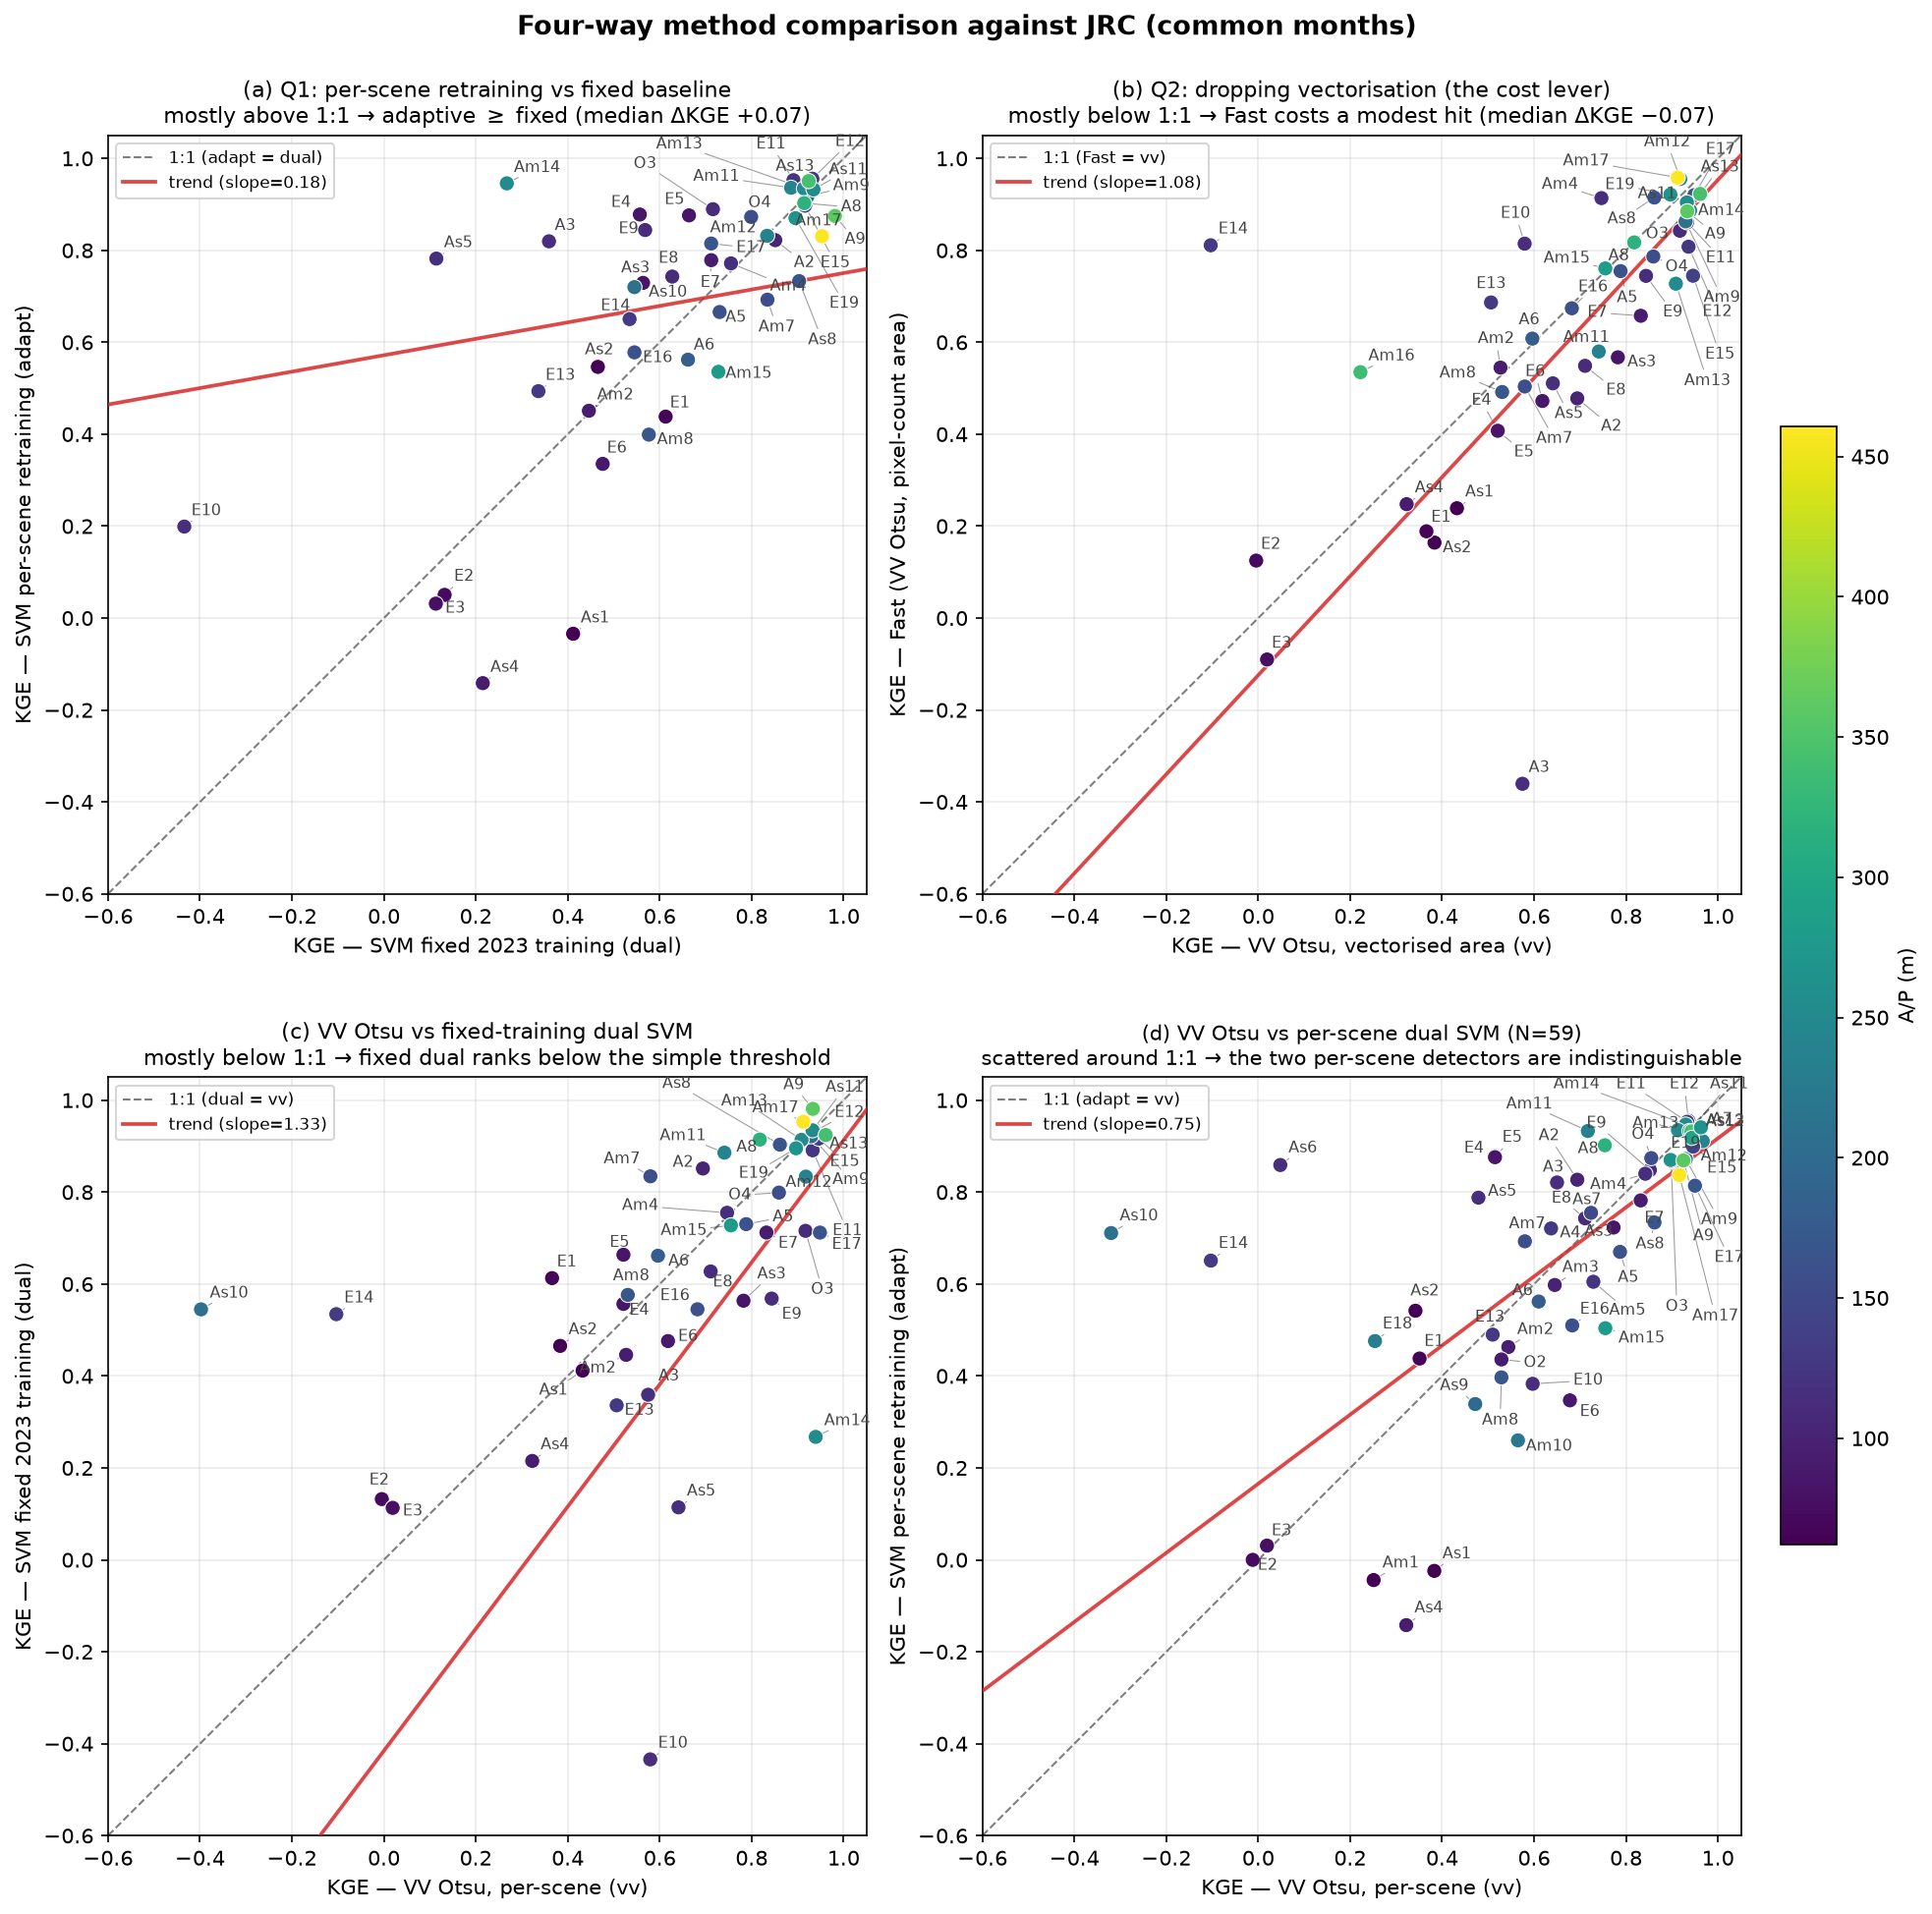
\includegraphics[width=\linewidth]{kge_4way}
  \caption{Four-detector KGE paired 1:1 against JRC. (a)--(c) use the
  47-reservoir subset with exports for all four detectors. (a) Per-scene
  retraining raises the dual SVM's skill over its fixed-training baseline.
  (b) Dropping vectorisation costs the VV Otsu detector a modest amount of
  accuracy. (c) The fixed-training dual SVM ranks below the simple
  per-scene VV Otsu threshold, showing polarisation count alone is not
  what earns accuracy. (d) The paper's central comparison, VV Otsu versus
  the per-scene dual SVM, on the full 59-reservoir set (Section~4.2): the
  two scatter around the 1:1 line and are statistically indistinguishable.
  Points are labelled by the continent-coded ID listed against each
  reservoir's name in Table~\ref{tab:pilot}.}
  \label{fig:fourway}
\end{figure}

\subsection{Independent validation against PlanetScope near-truth}
\label{sec:res_sicily}

Validated against 3~m PlanetScope near-truth (free of JRC's own 30~m
mixed-pixel limitation, Section~\ref{sec:study_sicily}), four Sicilian reservoirs reproduce the main
findings (Figure~\ref{fig:sicily}). Mean KGE ranks per-scene SVM (0.80)
$\approx$ fixed dual (0.80) $>$ Otsu (0.71) $>$ no-vectorisation (0.65): the
per-scene detectors again lead, and dropping vectorisation again costs accuracy
(mean $\Delta$KGE $-0.05$). One reservoir, Ancipa, is an instructive extreme:
at the lowest A/P in this set the single-band Otsu \emph{floors} near 60~ha
while the true surface falls to $\sim$5~ha, and the dual-band SVM follows the
drawdown down ($\Delta$KGE $+0.33$). This shows that VH \emph{can} rescue the
mixed-pixel, low-water regime. It is, however, a single near-truth case at an
extreme, and the global set (Section~\ref{sec:res_fourway}) shows no systematic
dual-polarisation advantage, so we present it as a mechanism rather than a rule.

\begin{figure}[H]
  \centering
  
\includegraphics[width=\linewidth]{sicily_planet_validation}
  \caption{Surface-area time series of the four detectors against PlanetScope
  3~m near-truth for the Sicilian reservoirs. At the extreme low-A/P Ancipa the
  VV Otsu floors at low water while the dual-band SVM tracks the drawdown. The
  effect does not generalise across the global set.}
  \label{fig:sicily}
\end{figure}

\subsection{Computational cost favours the simple detector}
\label{sec:res_cost}

An audit of Earth Engine compute usage (EECU-seconds per task, paired by
reservoir, cache-confounded pairs removed) shows that cost is driven by
per-scene retraining, not by the number of polarisations
(Figure~\ref{fig:eecu}). Because cost is a property of the per-scene processing
itself rather than of the accuracy outcome, this audit draws on every
reservoir for which the relevant pair of tasks was run, a broader pool than the
62-reservoir accuracy set that includes candidates later dropped for other
reasons. Sample sizes are given per comparison below and include the full
global-expansion batch. Polarisation count alone is
cheap: a dual SVM trained once on a fixed year costs a median $0.72\times$ the
single-band VV Otsu ($n=76$), whose per-scene 256-bin histogram and threshold
search outweigh a fixed classifier. Making the dual classifier adapt, however,
requires re-training it on every scene, and this per-scene dual SVM is the most
expensive method, at $1.17\times$ the VV Otsu ($n=92$) and $1.60\times$ the
fixed-training dual ($n=79$). The full cost ordering, fixed dual ($0.72\times$)
$<$ fast ($0.74\times$, $n=76$) $<$ VV Otsu ($1.00\times$) $<$ per-scene dual
($1.17\times$), is close to the inverse of the
accuracy ordering (Section~\ref{sec:res_fourway}): the most accurate method on
the median, the per-scene SVM, is also the most expensive, while the
per-scene VV Otsu matches its accuracy at roughly 15\% lower cost. The
implications for method choice are discussed in Section~\ref{sec:discussion}.

\begin{figure}[H]
  \centering
  
\includegraphics[width=0.8\linewidth]{eecu_svm_vs_vv}
  \caption{Per-reservoir Earth Engine compute cost of the fixed-training dual
  SVM versus VV Otsu (log--log). Most points fall below the 1:1 line, so
  polarisation count alone is not the cost driver. The per-scene retraining that
  makes the dual classifier adapt, by contrast, makes it the most expensive
  method (Section~\ref{sec:res_cost}).}
  \label{fig:eecu}
\end{figure}

\subsection{Beyond geometry: wind is null, climate is a genuine secondary axis}
\label{sec:res_climate}

A/P bounds accuracy from geometry and is blind to radiometric effects, which
form a second axis. Wind, the most-cited radiometric failure mode, shows no
systematic effect for this dataset: testing the Bragg prediction
\citep{Valenzuela1978} that VV should under-detect water relative to the
dual-band SVM as wind rises, on the 47 reservoirs with wind data and both
per-scene detectors, gives $r(\text{wind}_{p90}, \Delta\text{KGE}) = -0.06$
($p = 0.68$, Spearman $\rho = -0.12$, $p = 0.43$, Figure~\ref{fig:wind}),
indistinguishable from zero and far from the correlation Bragg scattering
would require. This null result is unaffected by post-processing: repeating
the test with the no-vectorisation VV variant (Section~\ref{sec:methods_cost})
gives an equivalent result ($r=-0.06$, $p=0.67$), and the gap-filling step's
own benefit to VV does not scale with wind either ($r=-0.04$, $p=0.78$), so
post-processing is not masking a wind-driven vulnerability that per-pixel
classification alone would show. We therefore do not treat wind as a
predictor of which detector is preferable for the present set of reservoirs,
though this is a sample-specific finding rather than a general one
(Section~\ref{sec:disc_geo_radio}).

Climate is different. At comparable A/P, reservoirs in humid, vegetated
settings are tracked less well than those in arid or Mediterranean settings
(Figure~\ref{fig:biome}): median KGE is 0.88 for Mediterranean ($n=15$) and
0.85 for semi-arid/arid ($n=16$), against 0.72 for (sub)tropical ($n=19$) and
0.47 for temperate/continental ($n=12$). This residual, beyond what A/P
explains, is statistically significant ($p = 0.012$), and unlike the pooled
result in an earlier, smaller sample, it does not depend on any single
uncertain reservoir: the reservoirs entering this test have already passed the
reference-quality screen (Section~\ref{sec:val_global}), so the disagreement
between climate zones is not attributable to a noisier optical reference in
any one of them. We therefore treat the climate effect as a genuine, if
secondary, modulator of the geometric ceiling that A/P sets, distinct from
the wind mechanism, which the data reject. A biome-by-biome caveat remains:
the temperate/continental group's low median is driven disproportionately by
narrow, valley-confined hydropower reservoirs in central Europe, and whether
their difficulty reflects climate, geometry not fully captured by static A/P,
or reservoir operation (Section~\ref{sec:disc_limitations}) is not yet
resolved.

\begin{figure}[H]
  \centering
  
\includegraphics[width=0.9\linewidth]{delta_kge_vs_wind_global}
  \caption{Accuracy gap (dual-band SVM minus VV Otsu) versus ERA5 wind exposure
  for the 47 reservoirs with wind data, coloured by A/P. No relationship is
  visible. Wind does not predict which detector is more accurate. Points are
  labelled by the continent-coded ID listed against each reservoir's name in
  Table~\ref{tab:pilot}.}
  \label{fig:wind}
\end{figure}

\begin{figure}[H]
  \centering
  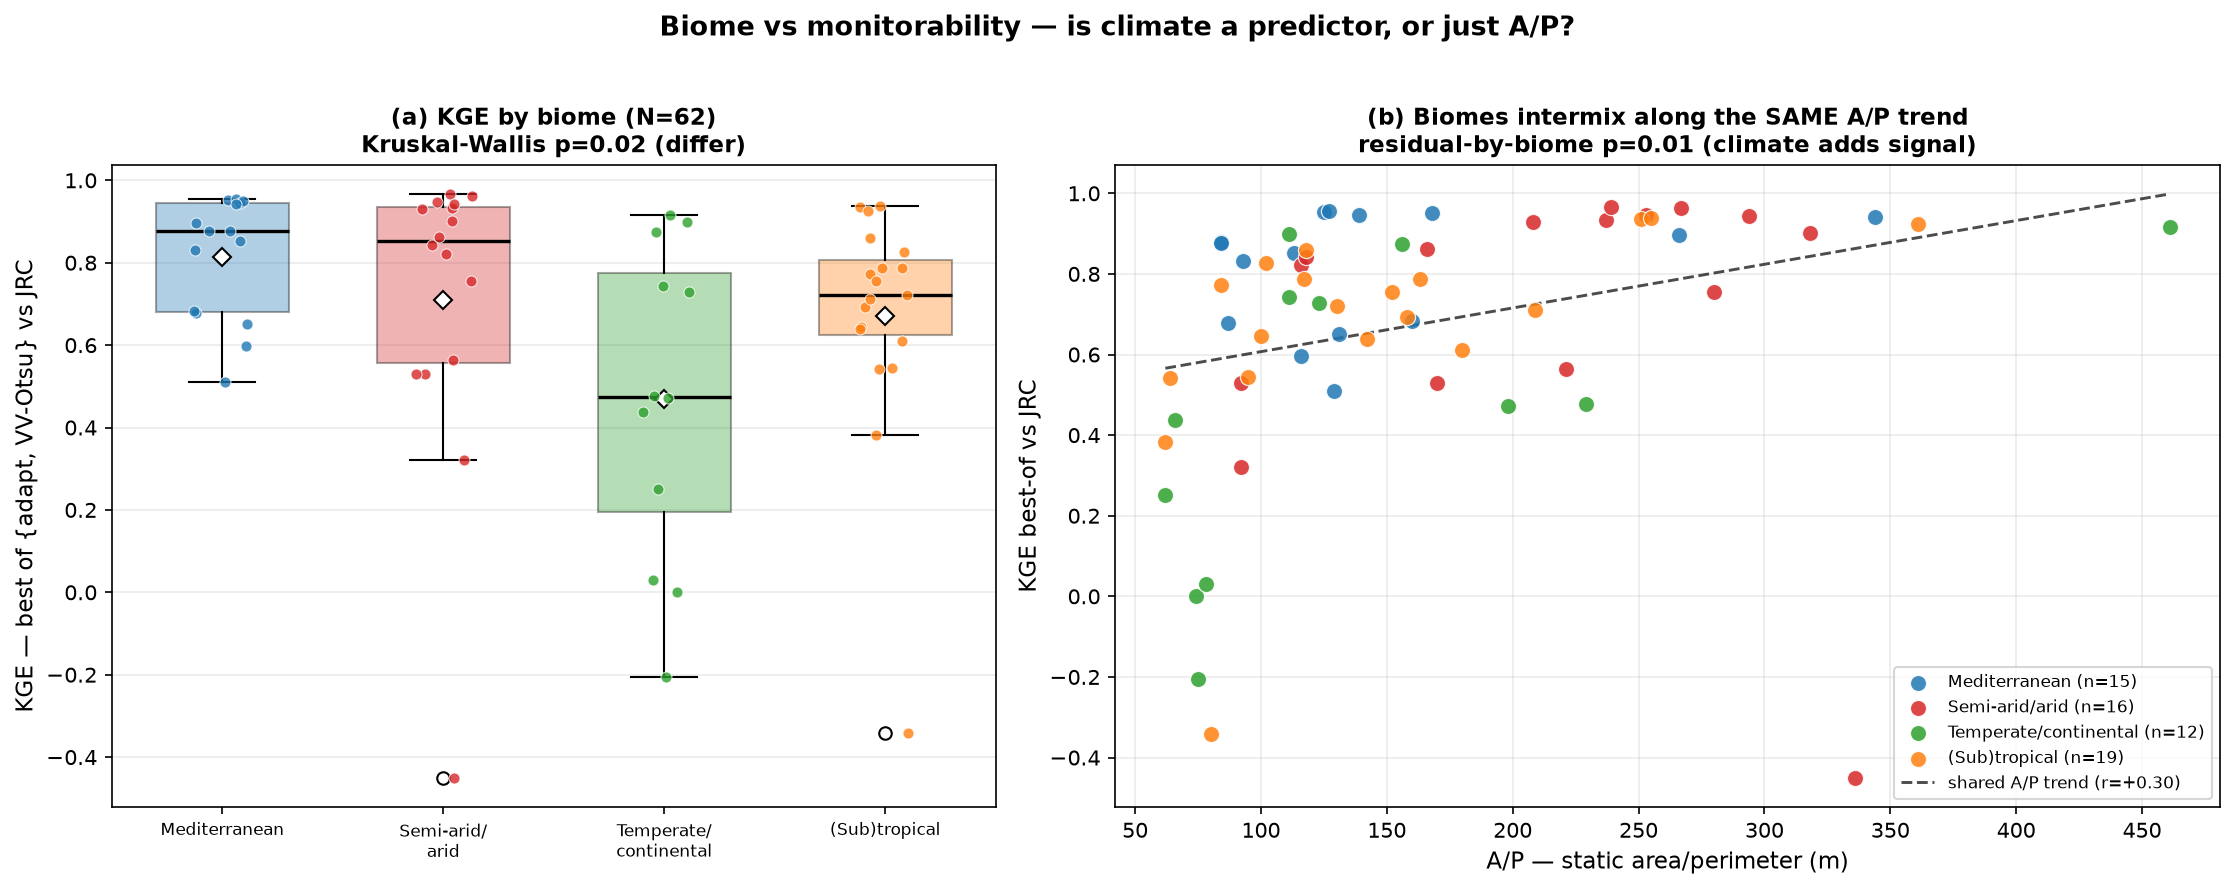
\includegraphics[width=\linewidth]{biome_kge}
  \caption{Surface-area skill by climate zone at comparable A/P, on the
  reference-quality-screened 62-reservoir set. Humid and vegetated settings
  (temperate, (sub)tropical) underperform arid and Mediterranean ones. The
  residual beyond A/P is significant ($p=0.012$) and, unlike in a smaller
  earlier sample, is not explained away by reference noise.}
  \label{fig:biome}
\end{figure}

The pooled A/P--KGE relationship (Section~\ref{sec:res_ap}) could in principle be
an artefact of which climates happen to sit at which A/P, rather than a
within-climate effect. It is largely not: tested separately within each biome
(Figure~\ref{fig:biome_ap}), A/P remains a predictor in the two zones with the
widest internal A/P spread, temperate/continental ($\rho = 0.68$, $p = 0.015$,
$n=12$) and (sub)tropical ($\rho = 0.62$, $p = 0.004$, $n=19$), and is weaker
and not significant in Mediterranean ($\rho = 0.26$, $p = 0.36$, $n=15$) and
semi-arid/arid ($\rho = 0.34$, $p = 0.19$, $n=16$) settings, where most
reservoirs already sit at high KGE regardless of A/P, leaving little residual
variance to correlate. A/P therefore predicts skill inside individual
climates, not only across the pooled sample, while climate independently
shifts the overall level.

\begin{figure}[H]
  \centering
  
\includegraphics[width=0.9\linewidth]{ap_kge_by_biome}
  \caption{A/P versus KGE within each climate zone, on the reference-quality-
  screened set. The relationship holds most clearly inside temperate/continental
  and (sub)tropical reservoirs, where A/P spans a wide range. In Mediterranean
  and semi-arid settings most reservoirs already reach high KGE, leaving little
  variance for A/P to explain.}
  \label{fig:biome_ap}
\end{figure}
